\chapter{Разработка онтологических моделей} \label{chapt2}

\section{Модель взаимодействия объектов системы электронного обучения} \label{sect2_1}

Данные в системе электронного обучения на основе семантических технологий хранятся в формате RDF. Для хранения данных в системе электронного обучения был разработан набор онтологий. В результате анализа учебных материалов, предметных областей и моделей существующих систем электронного обучения была разработана общая модель системы электронного обучения на основе семантических технологий. Разработанная модель данных системы электронного обучения обладает следующими важными характеристиками:

\begin{itemize}
\item возможность агрегации данных модели из сторонних источников;
\item динамическое связывание данных между различными уровнями и областями данных;
\item распределенное хранение и доступ к данным модели на разных уровнях и областях.
\end{itemize}

Модель данных системы электронного обучения условно делится на три основных уровня: 

\begin{itemize}
\item уровень предметных областей, 
\item уровень учебных материалов, 
\item уровень статистических данных по действиям пользователей в системе. 
\end{itemize}

Уровни модели связаны друг с другом для обеспечения взаимодействия различных ресурсов системы. Таким образом появляется возможность с помощью семантических связей между объектами различных уровней производить анализ предметных областей, учебных материалов и действий студентов в системе. Общая модель данных системы электронного обучения на основе семантических технологий представлена на рисунке \ref{img:overall_model}.

\begin{figure} [h] 
  \center
  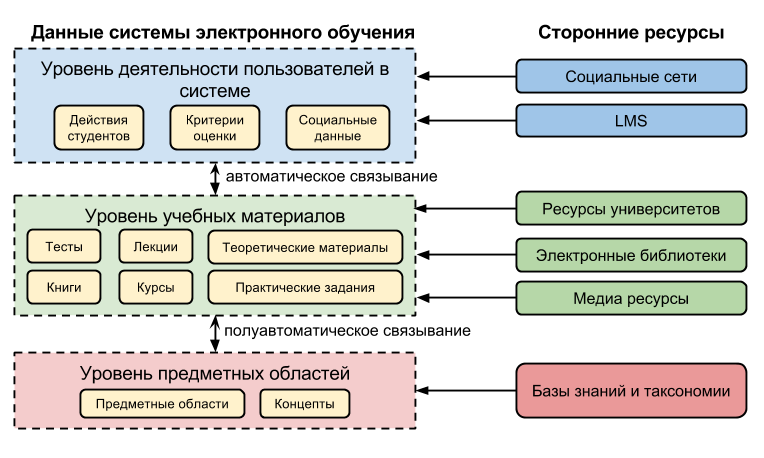
\includegraphics [width=0.95\textwidth] {overall_model}
  \caption{Общая модель данных системы электронного обучения на основе семантических технологий.} 
  \label{img:overall_model}  
\end{figure}

Уровень предметных областей является основой модели данных системы электронного обучения и содержит информацию о предметных областях науки и образования. На данном уровне хранится информация о концептах предметных областей и связях между ними. Концептом предметной области является концепт таксономии, метод, гипотеза, теорема или другой объект, использующийся в предметных областях наук и образовании. Сбор данных для этого уровня производится из сторонних баз знаний, таксономий и опубликованных наборов данных, таких как DBpedia, Yago, Freebase, WikiData и Mathematics Subject Classification. 

Уровень учебных материалов содержит информацию необходимую для проведения учебного процесса. Уровень содержит данные по структуре  образовательных программ, курсам, модулям, лекциям, теоретическому материалу, тестам, практическому материалу и медиа ресурсам. Сбор данных для этого уровня производится из хранилищ университетов, порталов MOOC проектов, открытых электронных библиотек и медиа ресурсов. Так же поддерживается возможность ручного создания и экспорта курсов с помощью средств редактирования онтологий, таких как Proteje \cite{jain2013ontology}. Связывание учебных материалов с концептами предметной области и областями производится в полуавтоматическом режиме. Для связывания объектов могут быть использованы алгоритмы обработки естественного языка. Использование данных алгоритмов позволяет извлекать из текста семантические объекты и создавать связи между ними. Одним из примеров такого связывания является поиск концептов предметной области в текстах заданий тестов и дальнейшее связывание найденных концептов с объектами заданий тестов. Также в модели поддерживается метод ручного связывания объектов на данном уровне.

Уровень статистических данных по действиям пользователей в системе содержит результаты обучения студентов и  данные по активности и действиям пользователей в системе и за ее пределами. Статистика ведется в системе управления обучением LMS(Learning Management System). LMS является основой системы управления учебной деятельностью и используется для разработки, управления и распространения учебных онлайн-материалов с обеспечением совместного доступа \cite{mahnegar2012learning}. При ведении статистики может быть использована информация из сторонних источников, таких как социальные сети. Данные о действиях пользователя из различных социальных сетей могут быть агрегированы в одну онтологию для создания более полной картины деятельности пользователя в сети и его коммуникации с другими пользователями. Связывание результатов обучения и статистических данных по действиям пользователей в системе с учебными материалами происходит в автоматическом режиме алгоритмами LMS. Данные связи позволяют производить анализ действий пользователя в системе и за ее пределами в проекции учебных материалов и предметных областей системы электронного обучения.

Разработанная модель данных системы электронного обучения на основе семантических технологий может быть реализована в виде онтологии, состоящей из набора модулей отвечающих за различные уровни и области данных модели. На основе описанной общей модели данных системы была разработана модульная онтология. Модульная онтология состоит из следующих модулей:

\begin{itemize}
\item Модуль учебных материалов - онтология, которая описывает отношения между курсами, модулями, лекциями, тестами, практиками и концептами предметной области;
\item Модуль тестов - онтология, которая подробно описывает содержание тестов, вопросы, ответы, варианты тестов;
\item Модуль деятельности и результатов студента в системе обучения - онтология, которая позволяет хранить статистику по действиям студентов в системе и результаты обучения студентов, включая правильные и неправильные ответы на тесты, прохождения лекций и результаты экзаменов.
\item Модуль оценки знаний студентов - онтология, которая позволяет хранить вычисленные автоматически оценки знаний студентов по определенным концептам и предметным областям.
\end{itemize} 

Разработанная модель позволяет расширять область своего покрытия и детализации областей и уровней системы электронного обучения путем создания и интеграции дополнительных модулей онтологии.



\section{Онтология учебных материалов} \label{sect2_2}

Онтология учебных материалов описывает отношения между курсами, модулями, лекциями, тестами, практиками и предметными областями и концептами. Онтология основана на  <<верхнеуровневых>> онтологиях рекомендованных к использованию при описании учебных материалов.

The Academic Institution Internal Structure Ontology (AIISO) является онтологией, описывающей внутреннюю организационную структуру образовательного процесса. AIISO предоставляет классы и свойства для описания курсов, модулей, практических и теоретических учебных материалов.

The Bibliographic Ontology (BIBO) является онтологией описывающей библиографические ресурсы. В онтологии учебных материалов BIBO используется для описания рекомендованной литературы, научных публикаций, методичек и монографий. 

The Ontology for Media Resources (MA-ONT) является онтологией описывающей медиа ресурсы. С помощью классов и свойств MA-ONT в онтологии учебных материалов производится связывание лекций с видео материалами.

Основными классами онтологии учебных материалов являются:

\begin{itemize}
\item Курс, 
\item Модуль, 
\item Лекция, 
\item Тест, 
\item Экзамен, 
\item Практика, 
\item Предметная область, 
\item Предметный термин (Концепт), 
\item Ресурс.
\end{itemize}

Онтология состоит из 32 классов, 42 объектных свойств и 13 свойств-значений. Модель онтологии учебных материалов представлена в приложении \ref{APP_A_EDU}.

В основе онтологии учебных материалов лежит модуль предметных областей и концептов. В данном модуле описываются отношения между концептами и объектами онтологии учебных материалов. В модуле описывается ряд вспомогательных классов и свойств для реализации методов гармонизации и анализа данных системы электронного обучения. Модель онтологии концептов и предметных областей представлена на рисунке \ref{img:ontology_term}.  

\begin{figure} [h] 
  \center
  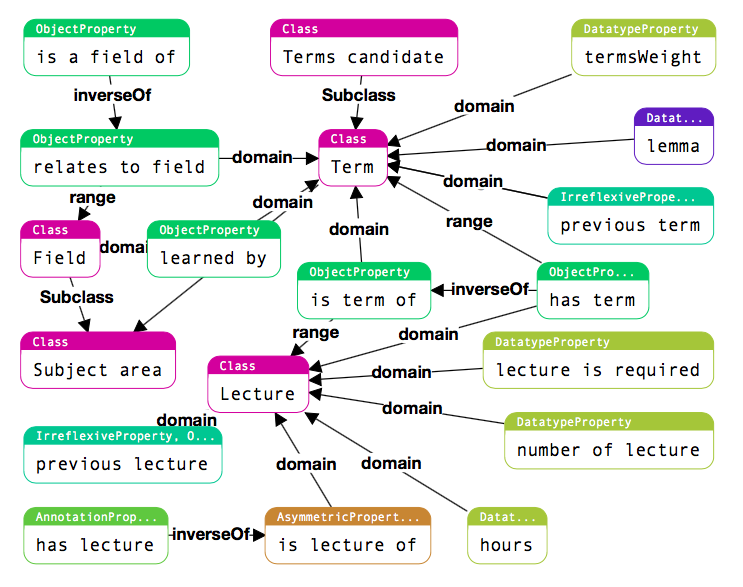
\includegraphics [width=0.95\textwidth] {ontology_term}
  \caption{Модель онтологии концептов и предметных областей.} 
  \label{img:ontology_term}  
\end{figure}

Разработанный модуль онтологии позволяет описывать предметные области, изучаемые в электронных курсах, используя готовые базы знаний и таксономии. Модуль содержит информацию об отношениях между концептами предметной области, что позволяет производить анализ содержания предметной области и на основе данного анализа производить анализ содержания учебных материалов и действий студентов в контексте предметных областей.  

Одной из главных особенностей разработанной онтологии является возможность произведения прямого и косвенного междисциплинарного связывания объектов в электронных курсах. Например, тест по курсу физики <<Интерференция и когерентность>> включает в себя использование математических концептов, таких как <<Вектор>> и <<Векторное произведение>>. Если студент не сможет успешно пройти данный тест, система должна рекомендовать к повторению не только лекции по физики, но и определенные лекции по векторной алгебре. Данный пример демонстрирует косвенное связывание курсов физики и векторной алгебры с помощью концептов предметной области  <<Вектор>> и <<Векторное произведение>>. Описанный пример представлен на рисунке \ref{img:ontology_edu_example}. Связывание объектов курса с концептами предметных областей позволяет косвенно связывать лекции, тесты и методические материалы друг с другом.

\begin{figure} [h] 
  \center
  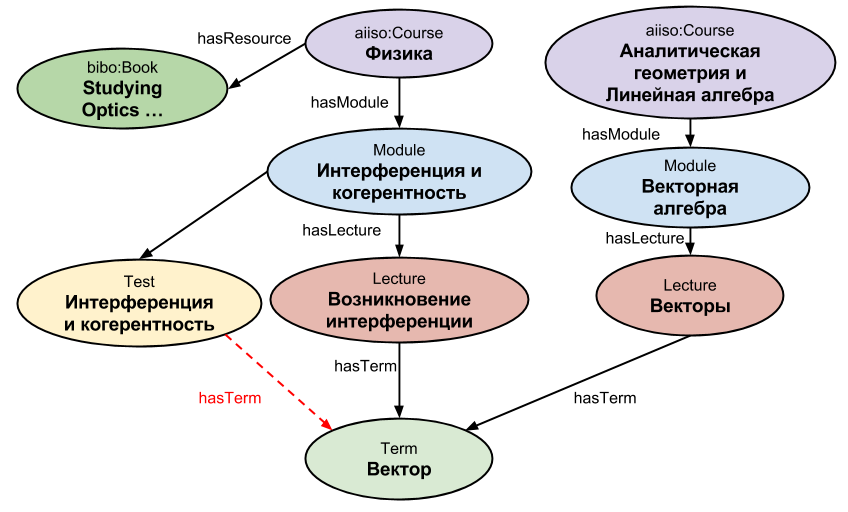
\includegraphics [width=0.95\textwidth] {ontology_edu_example}
  \caption{Пример косвенного связывания курсов с помощью концептов предметной области.} 
  \label{img:ontology_edu_example}  
\end{figure}

Косвенное связывание в онтологии учебных материалов позволяет оценивать покрытие тестами лекций электронного курса. С помощью использования косвенного связывания появляется возможность на основе анализа связей подбирать реллевантный учебный материал и находить похожие по содержанию электронные курсы. Подробный пример косвенного связывания тестов, лекций и курсов представлен в приложении \ref{APP_A_EXMPL}.   

Одной из задач технологии Linked Data является поддержка связей и отношений между различными наборами данных и источниками, использующими различные онтологии. Для семантической интеграции данных в онтологию учебных материалов было произведено отражение онтологий. Отображение онтологий — это процесс установления соответствий между понятиями нескольких онтологий. Отражение онтологий в разрабатываемой онтологии позволяет увеличить количество систем и ресурсов, поддерживающих данную онтологию.

Одним из опубликованных и релевантных словарей для описания учебных материалов является онтология TEACH (Teaching Core Vocabulary) \cite{kauppinen2012teaching}. TEACH облегченный словарь позволяющий преподавателям связывать объекты электронных курсов. Данный словарь был выбран для реализации отражения онтологии в онтологии учебных материалов.

Отражение онтологий производилось вручную на основе спецификации словаря TEACH. Эквивалентные классы двух онтологий связывались друг с другом с помощью свойства <<owl:equivalentClass>>. Эквивалентные свойства двух онтологий связывались друг с другом с помощью свойства <<owl:equivalentProperty>>.

Результаты отображения онтологии TEACH в онтологии учебных материалов представлены в таблице \ref{table:teach_mapping}. 

\begin{table}[ht]
\centering
\caption{Результаты отображения онтологии TEACH в онтологии учебных материалов.}
\label{table:teach_mapping}
\setlength{\tabcolsep}{10pt} 
\renewcommand{\arraystretch}{1.5} 
\begin{tabular}{ |c|c|  }
\hline Онтология учебных материалов  &  Teaching Core Vocabulary  \\
\hline \hline \multicolumn{2}{|c|}{Классы} \\ 
\hline aiiso:Course & teach:Course \\
\hline Resource & teach:Material \\
\hline Lecture & teach:Lecture \\
\hline \hline \multicolumn{2}{|c|}{Свойства} \\ 
\hline hasTeacher & teach:teacher \\
\hline isTeacherOf & teach:teacherOf \\
\hline
\end{tabular}
\end{table}



\section{Онтология тестов} \label{sect2_3}

Для детального описания содержания тестов был разработана онтология тестов. Онтология тестов является модулем онтологии системы электронного обучения, интегрированным в основную онтологию с целью детализации области тестов электронного курса. Разработка онтологии производилась методом раскрытия и конкретизации существующих онтологий верхнего уровня. Именно поэтому при разработке онтологии использовался нисходящий подход. Разработка онтологии велась на основе анализа существующих аналогов онтологий тестов и на основе разбора структуры наборов тестов предоставленных Университетом ИТМО.

Основными классами онтологии тестов являются:

\begin{itemize}
\item Тест,
\item Группа заданий (Вариант),
\item Задание,
\item Типизированный вопрос,
\item Типизированный ответ.
\end{itemize}

Онтология содержит 12 классов, 10 объектных свойств и 6 свойств-значений. Модель онтологии тестов представлена в приложении \ref{APP_A_TEST}.

Основной целью онтологии тестов является представление структуры тестов и предоставление возможности автоматического семантического связывания заданий тестов с концептами предметной области. Онтология описывает тест как набор из вариантов групп заданий. В каждой группе содержится набор заданий. Задания теста состоят из вопроса и набора ответов. В зависимости от типа вопроса у задания может быть различный набор правильных и неправильных ответов.

Онтология тестов является модулем онтологии учебных материалов. Онтология тестов интегрированная в онтологию учебных материалов и детализирует структуру объектов онтологии учебных материалов обладающих классом <<Тест>>. Аналогично в онтологии учебных материалов могут быть детализированы другие объекты, такие как <<Практика>>, <<Экзамен>> или <<Лекция>>. Основные объекты онтологии учебных материалов с интегрированным модулем онтологии тестов представлены на рисунке \ref{img:ontology_edu_test}.  

\begin{figure} [h] 
  \center
  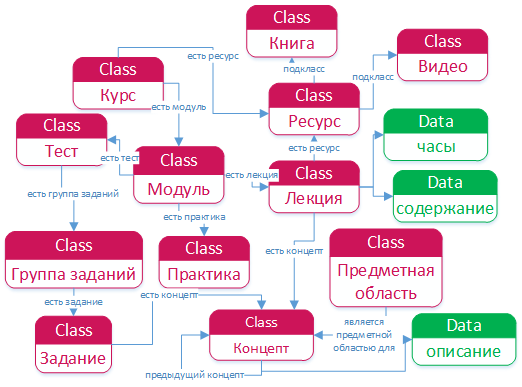
\includegraphics [width=0.95\textwidth] {ontology_edu_test}
  \caption{Основные объекты онтологии учебных материалов с интегрированным модулем онтологии тестов.} 
  \label{img:ontology_edu_test}  
\end{figure}

Связывание концептов предметной области с заданиями позволяет описать содержание вопроса и ответов задания. На основе данного описания может быть построен анализ ответов студентов на тесты электронного курса. 



\section{Онтология действий студента в системе электронного обучения} \label{sect2_4}

Онтология действий студента в системе электронного обучения была разработана для хранения информации о действиях, прогрессе и результатах обучения студентов в системе электронного обучения. При разработке были использованы  онтологии верхнего уровня: 

\begin{itemize}
\item онтология учебных материалов,
\item онтология тестов,
\item онтология Friend Of A Friend (FOAF).
\end{itemize}

Онтология FOAF определяет некоторые выражения, используемые в высказываниях о ком-либо, например: имя, пол и другие характеристики. Онтология FOAF используется для описания людей и отношений между ними. В электронной системе обучения FOAF может быть использована для описания персоналий студентов, преподавателей и других пользователей системы.

Основной задачей онтологии действий студента в системе электронного обучения является хранение действий студентов в системе. В онтологию может быть записана информация о просмотре студентом видео-лекции, о прохождении теста или завершении курса. Онтология действий студента в системе электронного обучения хранит в себе персональные данные студентов. В онтологию включены классы описывающие результаты студентов при прохождении тестов и изучении теоретического материала.

Основными классами онтологии учебных материалов являются:

\begin{itemize}
\item Студент,
\item Результат обучения,
\item Прогресс обучения,
\item Попытка сдачи теста,
\item Элемент теста.
\end{itemize}

Онтология действий студента в системе электронного обучения состоит из 10 классов, 15 объектных свойств и 5 свойств-значений. Модель действий студента в системе электронного обучения представлена в приложении \ref{APP_A_ACTION}.

Для хранения в онтологии действий студента в системе электронного обучения данных о прохождении студентом теоретического материала и лекций электронного курса используется связывания объектов онтологии с объектами онтологии учебных материалов. Для хранения в онтологии  ответов на тесты конкретного студента используется связывание с онтологией тестов. Связи между студентами, их ответами на задания тестов и  концептами предметной области позволяют создавать косвенные связи между студентом и объектами курса. На основе полученных косвенных связей возможно реализация персонализированной рекомендательной системы для корректировки процесса обучения студентов. 

На основе данных из онтологии действий студента в системе электронного обучения возможна реализация модулей анализа действий пользователя в системе электронного обучения. После прохождения теста студент может получить не только оценку, но и список концептов предметной области и материалов для повторения составленный на основе его ответов на тест электронного курса.



\section{Онтология оценки знаний студента} \label{sect2_5}

Для реализации методов автоматизированной оценки рейтингов и знаний студентов концептов и предметных областей был разработан и интегрирован в онтологическую модель системы электронного обучения модуль оценки знаний студентов. Модуль оценки знаний студентов - это онтология, которая позволяет хранить вычисленные автоматически рейтинги и оценки знаний студентов по определенным концептам и предметным областям. 

Основными классами онтологии оценки знаний студента являются:

\begin{itemize}
\item Оценка,
\item Рейтинг предметной области,
\item Рейтинг концепта предметной области.
\end{itemize}

Онтология оценки знаний студента состоит из 8 классов, 10 объектных свойств и 1 свойства-значения. Модель онтологии оценки знаний студента  представлена в приложении \ref{APP_A_KNOW}.

Онтология модуля содержит класс <<Rate>> (Оценка) и 5 подклассов, которые описывают следующие разновидности оценки:

\begin{itemize}
\item <<Lecture Term Rate>> - оценка концепта предметной области в контексте лекций; 
\item <<Test Attempt Term Rate>> - оценка концепта предметной области в контексте прохождения одного теста;
\item <<Average Test Term Rate>> - средняя оценка концепта предметной области за все тесты;
\item <<Total Term Rate>> - общая оценка концепта предметной области; 
\item <<Domain Rate>> - оценка предметной области. 
\end{itemize}

Каждый из классов оценки обладает свойством для хранения цифрового значения оценки <<value>>. Также онтология содержит объектные свойства для связывания объектов оценок с объектами студентов из модуля деятельности и результатов студента в системе обучения. В онтологии содержатся объектные свойства для связывания объектов тестов из модуля тестов с объектами концептов из модуля учебных материалов. Разработанная онтология позволяет добавлять новые классы оценок для хранения новых показателей при изменении алгоритмов расчета оценок.

Модуль онтологии оценки знаний студента интегрирован в онтологию действий студентов в системе электронного обучения. Данная интеграция позволяет связывать действия студентов по прохождению теоретического материала с показателями оценки знаний студентов. На основе связей между данными модулями онтологий производится оценка и хранение результатов обучения студентов системы электронного обучения. Основные объекты онтологии действий студентов в системе электронного обучения с интегрированным модулем онтологии оценки знаний студента представлены на рисунке \ref{img:ontology_action_know}.  

\begin{figure} [h] 
  \center
  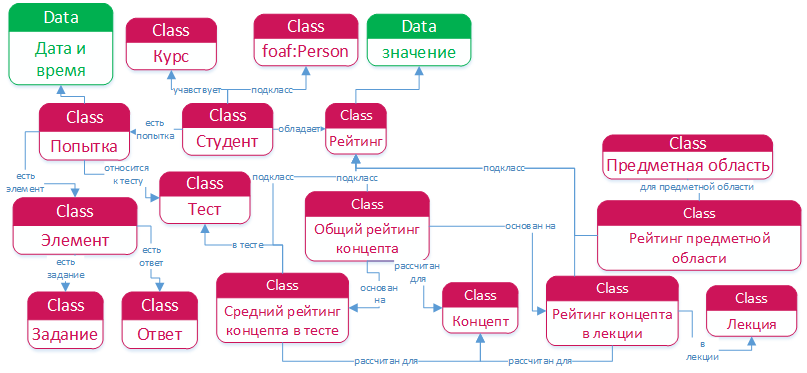
\includegraphics [width=0.95\textwidth] {ontology_action_know}
  \caption{Основные объекты онтологии действий студентов в системе электронного обучения с интегрированным модулем онтологии оценки знаний студента.} 
  \label{img:ontology_action_know}  
\end{figure}

